% Options for packages loaded elsewhere
\PassOptionsToPackage{unicode}{hyperref}
\PassOptionsToPackage{hyphens}{url}
\PassOptionsToPackage{dvipsnames,svgnames*,x11names*}{xcolor}
%
\documentclass[
]{article}
\usepackage{amsmath,amssymb}
\usepackage{lmodern}
\usepackage{ifxetex,ifluatex}
\ifnum 0\ifxetex 1\fi\ifluatex 1\fi=0 % if pdftex
  \usepackage[T1]{fontenc}
  \usepackage[utf8]{inputenc}
  \usepackage{textcomp} % provide euro and other symbols
\else % if luatex or xetex
  \usepackage{unicode-math}
  \defaultfontfeatures{Scale=MatchLowercase}
  \defaultfontfeatures[\rmfamily]{Ligatures=TeX,Scale=1}
\fi
% Use upquote if available, for straight quotes in verbatim environments
\IfFileExists{upquote.sty}{\usepackage{upquote}}{}
\IfFileExists{microtype.sty}{% use microtype if available
  \usepackage[]{microtype}
  \UseMicrotypeSet[protrusion]{basicmath} % disable protrusion for tt fonts
}{}
\makeatletter
\@ifundefined{KOMAClassName}{% if non-KOMA class
  \IfFileExists{parskip.sty}{%
    \usepackage{parskip}
  }{% else
    \setlength{\parindent}{0pt}
    \setlength{\parskip}{6pt plus 2pt minus 1pt}}
}{% if KOMA class
  \KOMAoptions{parskip=half}}
\makeatother
\usepackage{xcolor}
\IfFileExists{xurl.sty}{\usepackage{xurl}}{} % add URL line breaks if available
\IfFileExists{bookmark.sty}{\usepackage{bookmark}}{\usepackage{hyperref}}
\hypersetup{
  pdftitle={Week 3 - Homework},
  pdfauthor={STAT 420, Summer 2021, D. Unger},
  colorlinks=true,
  linkcolor=Maroon,
  filecolor=Maroon,
  citecolor=Blue,
  urlcolor=cyan,
  pdfcreator={LaTeX via pandoc}}
\urlstyle{same} % disable monospaced font for URLs
\usepackage[margin=1in]{geometry}
\usepackage{color}
\usepackage{fancyvrb}
\newcommand{\VerbBar}{|}
\newcommand{\VERB}{\Verb[commandchars=\\\{\}]}
\DefineVerbatimEnvironment{Highlighting}{Verbatim}{commandchars=\\\{\}}
% Add ',fontsize=\small' for more characters per line
\usepackage{framed}
\definecolor{shadecolor}{RGB}{248,248,248}
\newenvironment{Shaded}{\begin{snugshade}}{\end{snugshade}}
\newcommand{\AlertTok}[1]{\textcolor[rgb]{0.94,0.16,0.16}{#1}}
\newcommand{\AnnotationTok}[1]{\textcolor[rgb]{0.56,0.35,0.01}{\textbf{\textit{#1}}}}
\newcommand{\AttributeTok}[1]{\textcolor[rgb]{0.77,0.63,0.00}{#1}}
\newcommand{\BaseNTok}[1]{\textcolor[rgb]{0.00,0.00,0.81}{#1}}
\newcommand{\BuiltInTok}[1]{#1}
\newcommand{\CharTok}[1]{\textcolor[rgb]{0.31,0.60,0.02}{#1}}
\newcommand{\CommentTok}[1]{\textcolor[rgb]{0.56,0.35,0.01}{\textit{#1}}}
\newcommand{\CommentVarTok}[1]{\textcolor[rgb]{0.56,0.35,0.01}{\textbf{\textit{#1}}}}
\newcommand{\ConstantTok}[1]{\textcolor[rgb]{0.00,0.00,0.00}{#1}}
\newcommand{\ControlFlowTok}[1]{\textcolor[rgb]{0.13,0.29,0.53}{\textbf{#1}}}
\newcommand{\DataTypeTok}[1]{\textcolor[rgb]{0.13,0.29,0.53}{#1}}
\newcommand{\DecValTok}[1]{\textcolor[rgb]{0.00,0.00,0.81}{#1}}
\newcommand{\DocumentationTok}[1]{\textcolor[rgb]{0.56,0.35,0.01}{\textbf{\textit{#1}}}}
\newcommand{\ErrorTok}[1]{\textcolor[rgb]{0.64,0.00,0.00}{\textbf{#1}}}
\newcommand{\ExtensionTok}[1]{#1}
\newcommand{\FloatTok}[1]{\textcolor[rgb]{0.00,0.00,0.81}{#1}}
\newcommand{\FunctionTok}[1]{\textcolor[rgb]{0.00,0.00,0.00}{#1}}
\newcommand{\ImportTok}[1]{#1}
\newcommand{\InformationTok}[1]{\textcolor[rgb]{0.56,0.35,0.01}{\textbf{\textit{#1}}}}
\newcommand{\KeywordTok}[1]{\textcolor[rgb]{0.13,0.29,0.53}{\textbf{#1}}}
\newcommand{\NormalTok}[1]{#1}
\newcommand{\OperatorTok}[1]{\textcolor[rgb]{0.81,0.36,0.00}{\textbf{#1}}}
\newcommand{\OtherTok}[1]{\textcolor[rgb]{0.56,0.35,0.01}{#1}}
\newcommand{\PreprocessorTok}[1]{\textcolor[rgb]{0.56,0.35,0.01}{\textit{#1}}}
\newcommand{\RegionMarkerTok}[1]{#1}
\newcommand{\SpecialCharTok}[1]{\textcolor[rgb]{0.00,0.00,0.00}{#1}}
\newcommand{\SpecialStringTok}[1]{\textcolor[rgb]{0.31,0.60,0.02}{#1}}
\newcommand{\StringTok}[1]{\textcolor[rgb]{0.31,0.60,0.02}{#1}}
\newcommand{\VariableTok}[1]{\textcolor[rgb]{0.00,0.00,0.00}{#1}}
\newcommand{\VerbatimStringTok}[1]{\textcolor[rgb]{0.31,0.60,0.02}{#1}}
\newcommand{\WarningTok}[1]{\textcolor[rgb]{0.56,0.35,0.01}{\textbf{\textit{#1}}}}
\usepackage{longtable,booktabs,array}
\usepackage{calc} % for calculating minipage widths
% Correct order of tables after \paragraph or \subparagraph
\usepackage{etoolbox}
\makeatletter
\patchcmd\longtable{\par}{\if@noskipsec\mbox{}\fi\par}{}{}
\makeatother
% Allow footnotes in longtable head/foot
\IfFileExists{footnotehyper.sty}{\usepackage{footnotehyper}}{\usepackage{footnote}}
\makesavenoteenv{longtable}
\usepackage{graphicx}
\makeatletter
\def\maxwidth{\ifdim\Gin@nat@width>\linewidth\linewidth\else\Gin@nat@width\fi}
\def\maxheight{\ifdim\Gin@nat@height>\textheight\textheight\else\Gin@nat@height\fi}
\makeatother
% Scale images if necessary, so that they will not overflow the page
% margins by default, and it is still possible to overwrite the defaults
% using explicit options in \includegraphics[width, height, ...]{}
\setkeys{Gin}{width=\maxwidth,height=\maxheight,keepaspectratio}
% Set default figure placement to htbp
\makeatletter
\def\fps@figure{htbp}
\makeatother
\setlength{\emergencystretch}{3em} % prevent overfull lines
\providecommand{\tightlist}{%
  \setlength{\itemsep}{0pt}\setlength{\parskip}{0pt}}
\setcounter{secnumdepth}{-\maxdimen} % remove section numbering
\ifluatex
  \usepackage{selnolig}  % disable illegal ligatures
\fi

\title{Week 3 - Homework}
\author{STAT 420, Summer 2021, D. Unger}
\date{}

\begin{document}
\maketitle

\begin{center}\rule{0.5\linewidth}{0.5pt}\end{center}

\hypertarget{exercise-1-using-lm-for-inference}{%
\subsection{\texorpdfstring{Exercise 1 (Using \texttt{lm} for
Inference)}{Exercise 1 (Using lm for Inference)}}\label{exercise-1-using-lm-for-inference}}

For this exercise we will use the \texttt{cats} dataset from the
\texttt{MASS} package. You should use \texttt{?cats} to learn about the
background of this dataset.

\textbf{(a)} Fit the following simple linear regression model in
\texttt{R}. Use heart weight as the response and body weight as the
predictor.

\[
Y_i = \beta_0 + \beta_1 x_i + \epsilon_i
\]

Store the results in a variable called \texttt{cat\_model}. Use a \(t\)
test to test the significance of the regression. Report the following:

\begin{itemize}
\tightlist
\item
  The null and alternative hypotheses
\item
  The value of the test statistic
\item
  The p-value of the test
\item
  A statistical decision at \(\alpha = 0.05\)
\item
  A conclusion in the context of the problem
\end{itemize}

When reporting these, you should explicitly state them in your document,
not assume that a reader will find and interpret them from a large block
of \texttt{R} output.

\textbf{Solution}

\begin{Shaded}
\begin{Highlighting}[]
\NormalTok{cats }\OtherTok{\textless{}{-}}\NormalTok{ MASS}\SpecialCharTok{::}\NormalTok{cats}
\NormalTok{cat\_model }\OtherTok{\textless{}{-}} \FunctionTok{lm}\NormalTok{(Hwt }\SpecialCharTok{\textasciitilde{}}\NormalTok{ Bwt, }\AttributeTok{data =}\NormalTok{ cats)}
\end{Highlighting}
\end{Shaded}

Since we are trying to prove/disprove a linear relationship between the
predictor \texttt{(Bwt)} and the response \texttt{(Hwt)}, the null and
alternative hypothesis for \(\beta_1\) is:

\(H_0: \beta_1 = 0\) vs \(H_1: \beta_1 \neq 0\)

The following table shows some of the coefficients for the model:

\begin{Shaded}
\begin{Highlighting}[]
\FunctionTok{library}\NormalTok{(knitr)}

\NormalTok{coef\_cat }\OtherTok{\textless{}{-}} \FunctionTok{summary}\NormalTok{(cat\_model)}\SpecialCharTok{$}\NormalTok{coefficients}
\NormalTok{coef\_table }\OtherTok{\textless{}{-}} \FunctionTok{data.frame}\NormalTok{(}
  \AttributeTok{row.names =} \FunctionTok{c}\NormalTok{(}\StringTok{"Beta\_0\_hat"}\NormalTok{, }\StringTok{"Beta\_1\_hat"}\NormalTok{),}
  \StringTok{"Estimate"} \OtherTok{=} \FunctionTok{c}\NormalTok{(coef\_cat[}\DecValTok{1}\NormalTok{, }\DecValTok{1}\NormalTok{],}
\NormalTok{                  coef\_cat[}\DecValTok{2}\NormalTok{, }\DecValTok{1}\NormalTok{]),}
  \StringTok{"t value"} \OtherTok{=} \FunctionTok{c}\NormalTok{(coef\_cat[}\DecValTok{1}\NormalTok{, }\DecValTok{3}\NormalTok{],}
\NormalTok{                  coef\_cat[}\DecValTok{2}\NormalTok{, }\DecValTok{3}\NormalTok{]),}
  \StringTok{"p value"} \OtherTok{=} \FunctionTok{c}\NormalTok{(}\FunctionTok{formatC}\NormalTok{(coef\_cat[}\DecValTok{1}\NormalTok{, }\DecValTok{4}\NormalTok{],}\AttributeTok{format=}\StringTok{"e"}\NormalTok{),}
                  \FunctionTok{formatC}\NormalTok{(coef\_cat[}\DecValTok{2}\NormalTok{, }\DecValTok{4}\NormalTok{],}\AttributeTok{format=}\StringTok{"e"}\NormalTok{))  }
\NormalTok{)}

\FunctionTok{kable}\NormalTok{(coef\_table, }
      \AttributeTok{col.names =} \FunctionTok{c}\NormalTok{(}\StringTok{"Estimate "}\NormalTok{,}\StringTok{"t value"}\NormalTok{,}\StringTok{"p value"}\NormalTok{),}
      \AttributeTok{caption =} \StringTok{"Coefficients for Linear Model on MASS::cats dataset."}\NormalTok{)}
\end{Highlighting}
\end{Shaded}

\begin{longtable}[]{@{}lrrl@{}}
\caption{Coefficients for Linear Model on MASS::cats
dataset.}\tabularnewline
\toprule
& Estimate & t value & p value \\
\midrule
\endfirsthead
\toprule
& Estimate & t value & p value \\
\midrule
\endhead
Beta\_0\_hat & -0.3566624 & -0.5152019 & 6.0721e-01 \\
Beta\_1\_hat & 4.0340627 & 16.1193908 & 6.9690e-34 \\
\bottomrule
\end{longtable}

\begin{Shaded}
\begin{Highlighting}[]
\NormalTok{stat\_decide }\OtherTok{\textless{}{-}} \ControlFlowTok{function}\NormalTok{(p\_value, }\AttributeTok{alpha =} \FloatTok{0.01}\NormalTok{) \{}
  \FunctionTok{ifelse}\NormalTok{(p\_value }\SpecialCharTok{\textless{}}\NormalTok{ alpha, }\StringTok{"Reject the Null Hypothesis"}\NormalTok{, }\StringTok{"FTR the Null Hypothesis"}\NormalTok{)}
\NormalTok{\}}
\NormalTok{(beta\_10\_decision }\OtherTok{\textless{}{-}} \FunctionTok{stat\_decide}\NormalTok{(coef\_cat[}\DecValTok{2}\NormalTok{, }\DecValTok{4}\NormalTok{], }\AttributeTok{alpha =} \FloatTok{0.05}\NormalTok{))}
\end{Highlighting}
\end{Shaded}

\begin{verbatim}
## [1] "Reject the Null Hypothesis"
\end{verbatim}

\emph{Statistical decision at } \(\alpha = 0.05\) : \textbf{Reject the
Null Hypothesis}

Given that we reject the null hypothesis \(H_0: \beta_1 = 0\), we can
conclude that seems to be a considerable linear relationship between the
predictor \texttt{(Bwt)} and the response \texttt{(Hwt)}. In other
words, is reasonable to think that the \texttt{Body\ Weight} can explain
some of the variation observed in the \texttt{Heart\ Weight}.

\textbf{(b)} Calculate a 95\% confidence interval for \(\beta_1\). Give
an interpretation of the interval in the context of the problem.

\begin{Shaded}
\begin{Highlighting}[]
\NormalTok{(beta\_1\_interval }\OtherTok{\textless{}{-}} \FunctionTok{confint}\NormalTok{(cat\_model, }\AttributeTok{parm =} \StringTok{"Bwt"}\NormalTok{, }\AttributeTok{level =} \FloatTok{0.95}\NormalTok{))}
\end{Highlighting}
\end{Shaded}

\begin{verbatim}
##        2.5 %   97.5 %
## Bwt 3.539343 4.528782
\end{verbatim}

With \texttt{95\%} of confidence we can state: The \textbf{true value
for change in mean} of the \texttt{Heart\ Weight} that corresponds to an
increment of \texttt{1\ kg} of the \texttt{Body\ Weight} is located in
the interval: \(\left(3.539343, 4.528782\right)\)

On this basis we can also reject \(H_0: \beta_1 = 0\), since 0 is not in
the interval.

\textbf{(c)} Calculate a 90\% confidence interval for \(\beta_0\). Give
an interpretation of the interval in the context of the problem.

\begin{Shaded}
\begin{Highlighting}[]
\NormalTok{(beta\_0\_interval }\OtherTok{\textless{}{-}} \FunctionTok{confint}\NormalTok{(cat\_model, }\AttributeTok{parm =} \StringTok{"(Intercept)"}\NormalTok{, }\AttributeTok{level =} \FloatTok{0.9}\NormalTok{))}
\end{Highlighting}
\end{Shaded}

\begin{verbatim}
##                   5 %      95 %
## (Intercept) -1.502834 0.7895096
\end{verbatim}

With \texttt{90\%} of confidence we say that, for a cat with
\texttt{Body\ Weight} of \texttt{0\ Kg} the mean of the
\texttt{Heart\ Weight} is located in the interval:
\(\left(-1.502834, 0.7895096\right)\). Note that in real life the only
\texttt{Heart\ Weight} value that makes sense would be 0, which in this
case is in the \texttt{Confidence\ Interval}.

\textbf{(d)} Use a 90\% confidence interval to estimate the mean heart
weight for body weights of 2.1 and 2.8 kilograms. Which of the two
intervals is wider? Why?

\begin{Shaded}
\begin{Highlighting}[]
\NormalTok{(conf\_interval }\OtherTok{\textless{}{-}} \FunctionTok{predict}\NormalTok{(cat\_model, }\AttributeTok{newdata =} \FunctionTok{data.frame}\NormalTok{(}\AttributeTok{Bwt =} \FunctionTok{c}\NormalTok{(}\FloatTok{2.1}\NormalTok{, }\FloatTok{2.8}\NormalTok{)),}
        \AttributeTok{interval =} \FunctionTok{c}\NormalTok{(}\StringTok{"confidence"}\NormalTok{), }\AttributeTok{level =} \FloatTok{0.9}\NormalTok{))}
\end{Highlighting}
\end{Shaded}

\begin{verbatim}
##         fit       lwr       upr
## 1  8.114869  7.787882  8.441856
## 2 10.938713 10.735843 11.141583
\end{verbatim}

\begin{Shaded}
\begin{Highlighting}[]
\NormalTok{mean\_cats }\OtherTok{\textless{}{-}} \FunctionTok{c}\NormalTok{(}\FunctionTok{mean}\NormalTok{(cats}\SpecialCharTok{$}\NormalTok{Bwt), }\FunctionTok{mean}\NormalTok{(cats}\SpecialCharTok{$}\NormalTok{Hwt))}
\NormalTok{len\_interval\_21 }\OtherTok{\textless{}{-}}\NormalTok{ conf\_interval[}\DecValTok{1}\NormalTok{, }\DecValTok{3}\NormalTok{] }\SpecialCharTok{{-}}\NormalTok{ conf\_interval[}\DecValTok{1}\NormalTok{, }\DecValTok{2}\NormalTok{]}
\NormalTok{len\_interval\_28 }\OtherTok{\textless{}{-}}\NormalTok{ conf\_interval[}\DecValTok{2}\NormalTok{, }\DecValTok{3}\NormalTok{] }\SpecialCharTok{{-}}\NormalTok{ conf\_interval[}\DecValTok{2}\NormalTok{, }\DecValTok{2}\NormalTok{]}
\end{Highlighting}
\end{Shaded}

\emph{Length of the interval for Btw = 2.1:} 0.653974

\emph{Length of the interval for Btw = 2.8:} 0.4057402

\emph{\(\bar\x\)} : 2.7236111

The interval for 2.1 Kg is wider in this case because 2.1 is farther
from the mean of \texttt{x} (\texttt{Bwt}). We are less confident in
areas with fewer data points (i.e.~away from the mean), to account for
that, the interval has to be wider.

\textbf{(e)} Use a 90\% prediction interval to predict the heart weight
for body weights of 2.8 and 4.2 kilograms.

\begin{Shaded}
\begin{Highlighting}[]
\NormalTok{(pred\_interval }\OtherTok{\textless{}{-}} \FunctionTok{predict}\NormalTok{(cat\_model, }\AttributeTok{newdata =} \FunctionTok{data.frame}\NormalTok{(}\AttributeTok{Bwt =} \FunctionTok{c}\NormalTok{(}\FloatTok{2.8}\NormalTok{, }\FloatTok{4.2}\NormalTok{)),}
        \AttributeTok{interval =} \FunctionTok{c}\NormalTok{(}\StringTok{"prediction"}\NormalTok{), }\AttributeTok{level =} \FloatTok{0.9}\NormalTok{))}
\end{Highlighting}
\end{Shaded}

\begin{verbatim}
##        fit       lwr      upr
## 1 10.93871  8.525541 13.35189
## 2 16.58640 14.097100 19.07570
\end{verbatim}

\begin{Shaded}
\begin{Highlighting}[]
\NormalTok{pred\_table }\OtherTok{\textless{}{-}} \FunctionTok{data.frame}\NormalTok{(}
  \CommentTok{\#row.names = c("Beta\_0\_hat", "Beta\_1\_hat"),}
  \StringTok{"Body Weight"} \OtherTok{=} \FunctionTok{c}\NormalTok{(}\FloatTok{2.8}\NormalTok{,}
                  \FloatTok{4.2}\NormalTok{),}
  \StringTok{"Predicted Hwt"} \OtherTok{=} \FunctionTok{c}\NormalTok{(pred\_interval[}\DecValTok{1}\NormalTok{, }\DecValTok{1}\NormalTok{],}
\NormalTok{                  pred\_interval[}\DecValTok{2}\NormalTok{, }\DecValTok{1}\NormalTok{]),}
  \StringTok{"Lower Bound"} \OtherTok{=} \FunctionTok{c}\NormalTok{(pred\_interval[}\DecValTok{1}\NormalTok{, }\DecValTok{2}\NormalTok{],}
\NormalTok{                  pred\_interval[}\DecValTok{2}\NormalTok{, }\DecValTok{2}\NormalTok{]), }
  \StringTok{"Upper Bound"} \OtherTok{=} \FunctionTok{c}\NormalTok{(pred\_interval[}\DecValTok{1}\NormalTok{, }\DecValTok{3}\NormalTok{],}
\NormalTok{                  pred\_interval[}\DecValTok{2}\NormalTok{, }\DecValTok{3}\NormalTok{])   }
\NormalTok{)}

\FunctionTok{kable}\NormalTok{(pred\_table, }
      \AttributeTok{col.names =} \FunctionTok{c}\NormalTok{(}\StringTok{"Body Weight (kg)"}\NormalTok{,}\StringTok{"Predicted Hwt (g)"}\NormalTok{,}\StringTok{"Lower Bound"}\NormalTok{,}\StringTok{"Upper Bound"}\NormalTok{),}
      \AttributeTok{caption =} \StringTok{"90\% Prediction Intervals"}\NormalTok{)}
\end{Highlighting}
\end{Shaded}

\begin{longtable}[]{@{}rrrr@{}}
\caption{90\% Prediction Intervals}\tabularnewline
\toprule
Body Weight (kg) & Predicted Hwt (g) & Lower Bound & Upper Bound \\
\midrule
\endfirsthead
\toprule
Body Weight (kg) & Predicted Hwt (g) & Lower Bound & Upper Bound \\
\midrule
\endhead
2.8 & 10.93871 & 8.525541 & 13.35189 \\
4.2 & 16.58640 & 14.097100 & 19.07570 \\
\bottomrule
\end{longtable}

\textbf{(f)} Create a scatterplot of the data. Add the regression line,
95\% confidence bands, and 95\% prediction bands.

\begin{Shaded}
\begin{Highlighting}[]
\NormalTok{bwt\_seq }\OtherTok{\textless{}{-}} \FunctionTok{seq}\NormalTok{(}\FunctionTok{min}\NormalTok{(cats}\SpecialCharTok{$}\NormalTok{Bwt), }\FunctionTok{min}\NormalTok{(cats}\SpecialCharTok{$}\NormalTok{Hwt), }\FloatTok{0.02}\NormalTok{)}

\NormalTok{conf\_interval\_seq }\OtherTok{\textless{}{-}} \FunctionTok{predict}\NormalTok{(cat\_model, }\AttributeTok{newdata =} \FunctionTok{data.frame}\NormalTok{(}\AttributeTok{Bwt =}\NormalTok{ bwt\_seq),}
        \AttributeTok{interval =} \FunctionTok{c}\NormalTok{(}\StringTok{"confidence"}\NormalTok{), }\AttributeTok{level =} \FloatTok{0.95}\NormalTok{)}

\NormalTok{pred\_interval\_seq }\OtherTok{\textless{}{-}} \FunctionTok{predict}\NormalTok{(cat\_model, }\AttributeTok{newdata =} \FunctionTok{data.frame}\NormalTok{(}\AttributeTok{Bwt =}\NormalTok{ bwt\_seq),}
        \AttributeTok{interval =} \FunctionTok{c}\NormalTok{(}\StringTok{"prediction"}\NormalTok{), }\AttributeTok{level =} \FloatTok{0.95}\NormalTok{)}

\FunctionTok{plot}\NormalTok{(Hwt }\SpecialCharTok{\textasciitilde{}}\NormalTok{ Bwt, }\AttributeTok{data =}\NormalTok{ cats,}
     \AttributeTok{xlab =} \StringTok{"Body Weight (kg)"}\NormalTok{,}
     \AttributeTok{ylab =} \StringTok{"Heart Weight (g)"}\NormalTok{,}
     \AttributeTok{main =} \StringTok{"Heart Weight vs Body Weight"}\NormalTok{,}
     \AttributeTok{pch =} \DecValTok{20}\NormalTok{,}
     \AttributeTok{cex =} \DecValTok{2}\NormalTok{,}
     \AttributeTok{col =} \StringTok{"grey"}
     \CommentTok{\#ylim = c(min(pred\_interval\_seq), max(pred\_interval\_seq))}
\NormalTok{)}
\FunctionTok{abline}\NormalTok{(cat\_model, }\AttributeTok{lwd =} \DecValTok{3}\NormalTok{, }\AttributeTok{col =} \StringTok{"darkorange"}\NormalTok{)}

\FunctionTok{lines}\NormalTok{(bwt\_seq, conf\_interval\_seq[, }\StringTok{"lwr"}\NormalTok{], }\AttributeTok{col =} \StringTok{"dodgerblue"}\NormalTok{, }\AttributeTok{lwd =} \DecValTok{3}\NormalTok{, }\AttributeTok{lty =} \DecValTok{2}\NormalTok{)}
\FunctionTok{lines}\NormalTok{(bwt\_seq, conf\_interval\_seq[, }\StringTok{"upr"}\NormalTok{], }\AttributeTok{col =} \StringTok{"dodgerblue"}\NormalTok{, }\AttributeTok{lwd =} \DecValTok{3}\NormalTok{, }\AttributeTok{lty =} \DecValTok{2}\NormalTok{)}

\FunctionTok{lines}\NormalTok{(bwt\_seq, pred\_interval\_seq[, }\StringTok{"lwr"}\NormalTok{], }\AttributeTok{col =} \StringTok{"darkolivegreen3"}\NormalTok{, }\AttributeTok{lwd =} \DecValTok{3}\NormalTok{, }\AttributeTok{lty =} \DecValTok{4}\NormalTok{)}
\FunctionTok{lines}\NormalTok{(bwt\_seq, pred\_interval\_seq[, }\StringTok{"upr"}\NormalTok{], }\AttributeTok{col =} \StringTok{"darkolivegreen3"}\NormalTok{, }\AttributeTok{lwd =} \DecValTok{3}\NormalTok{, }\AttributeTok{lty =} \DecValTok{4}\NormalTok{)}

\FunctionTok{legend}\NormalTok{(}\StringTok{"topleft"}\NormalTok{, }\FunctionTok{c}\NormalTok{(}\StringTok{"Estimate"}\NormalTok{, }\StringTok{"Confidence Interval"}\NormalTok{, }\StringTok{"Prediction Interval"}\NormalTok{), }
       \AttributeTok{lty =} \FunctionTok{c}\NormalTok{(}\DecValTok{1}\NormalTok{, }\DecValTok{2}\NormalTok{, }\DecValTok{4}\NormalTok{),}
       \AttributeTok{lwd =} \DecValTok{3}\NormalTok{,}
       \AttributeTok{col =} \FunctionTok{c}\NormalTok{(}\StringTok{"darkorange"}\NormalTok{, }\StringTok{"dodgerblue"}\NormalTok{, }\StringTok{"darkolivegreen3"}\NormalTok{))}
\end{Highlighting}
\end{Shaded}

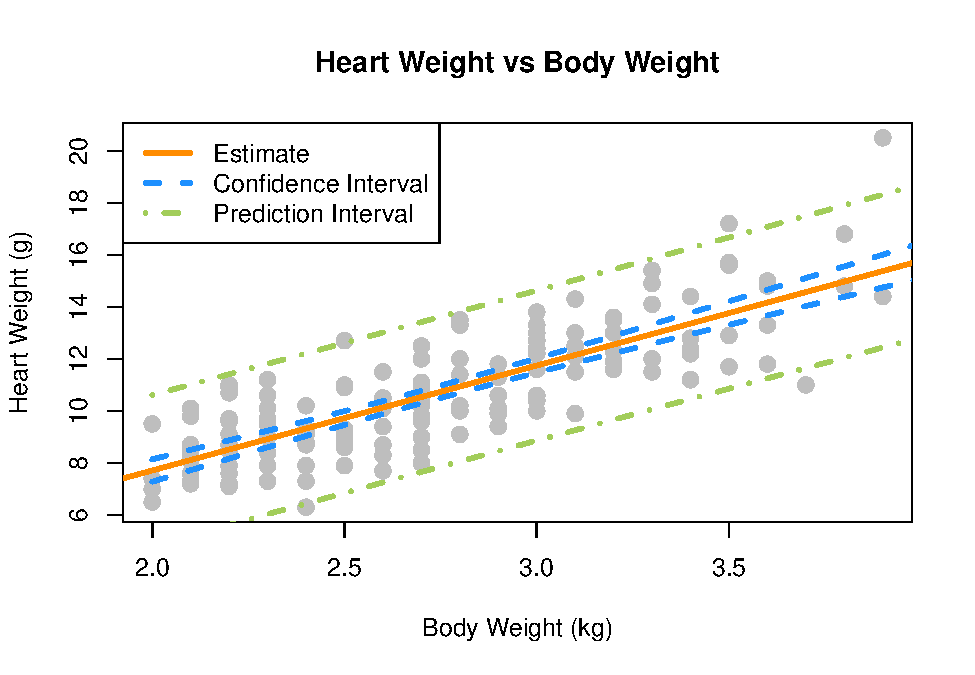
\includegraphics{w03-hw-ap41_files/figure-latex/unnamed-chunk-8-1.pdf}

\textbf{(g)} Use a \(t\) test to test:

\begin{itemize}
\tightlist
\item
  \(H_0: \beta_1 = 4\)
\item
  \(H_1: \beta_1 \neq 4\)
\end{itemize}

Report the following:

\begin{itemize}
\tightlist
\item
  The value of the test statistic
\item
  The p-value of the test
\item
  A statistical decision at \(\alpha = 0.05\)
\end{itemize}

When reporting these, you should explicitly state them in your document,
not assume that a reader will find and interpret them from a large block
of \texttt{R} output.

\begin{center}\rule{0.5\linewidth}{0.5pt}\end{center}

\end{document}
